% !Mode:: "TeX:UTF-8"
\documentclass{article}

%%%%%%%%------------------------------------------------------------------------
%%%% 日常所用宏包

%% 控制页边距
% 如果是beamer文档类, 则不用geometry
\makeatletter
\@ifclassloaded{beamer}{}{\usepackage[top=2.5cm, bottom=2.5cm, left=2.5cm, right=2.5cm]{geometry}}
\makeatother

%% 控制项目列表
\usepackage{enumerate}

%% 多栏显示
\usepackage{multicol}

%% 算法环境
\usepackage{algorithm}  
\usepackage{algorithmic} 
\usepackage{float} 

%% 网址引用
\usepackage{url}

%% 控制矩阵行距
\renewcommand\arraystretch{1.4}

%% hyperref宏包,生成可定位点击的超链接,并且会生成pdf书签
\makeatletter
\@ifclassloaded{beamer}{
\usepackage{hyperref}
}{
\usepackage[%
    pdfstartview=FitH,%
    CJKbookmarks=true,%
    bookmarks=true,%
    bookmarksnumbered=true,%
    bookmarksopen=true,%
    colorlinks=true,%
    citecolor=blue,%
    linkcolor=blue,%
    anchorcolor=green,%
    urlcolor=blue%
]{hyperref}
}
\makeatother



\makeatletter % 如果是 beamer 不需要下面两个包
\@ifclassloaded{beamer}{

}{
%% 控制标题
\usepackage{titlesec}
%% 控制目录
\usepackage{titletoc}
}
\makeatother

%% 控制表格样式
\usepackage{booktabs}

%% 控制字体大小
\usepackage{type1cm}

%% 首行缩进,用\noindent取消某段缩进
\usepackage{indentfirst}

%% 支持彩色文本、底色、文本框等
\usepackage{color,xcolor}

%% AMS LaTeX宏包: http://zzg34b.w3.c361.com/package/maths.htm#amssymb
\usepackage{amsmath,amssymb}

%%%% 基本插图方法
%% 图形宏包
\usepackage{graphicx}

%% 多个图形并排
\usepackage{subfig}

%%%% 基本插图方法结束

%%%% pgf/tikz绘图宏包设置
\usepackage{pgf,tikz}
\usetikzlibrary{shapes,automata,snakes,backgrounds,arrows}
\usetikzlibrary{mindmap}
%% 可以直接在latex文档中使用graphviz/dot语言,
%% 也可以用dot2tex工具将dot文件转换成tex文件再include进来
%% \usepackage[shell,pgf,outputdir={docgraphs/}]{dot2texi}
%%%% pgf/tikz设置结束


\makeatletter % 如果是 beamer 不需要下面两个包
\@ifclassloaded{beamer}{

}{
%%%% fancyhdr设置页眉页脚
%% 页眉页脚宏包
\usepackage{fancyhdr}
%% 页眉页脚风格
\pagestyle{plain}
}

%% 有时会出现\headheight too small的warning
\setlength{\headheight}{15pt}

%% 清空当前页眉页脚的默认设置
%\fancyhf{}
%%%% fancyhdr设置结束


\makeatletter % 对 beamer 要重新设置
\@ifclassloaded{beamer}{

}{
%%%% 设置listings宏包用来粘贴源代码
%% 方便粘贴源代码,部分代码高亮功能
\usepackage{listings}

%% 设置listings宏包的一些全局样式
%% 参考http://hi.baidu.com/shawpinlee/blog/item/9ec431cbae28e41cbe09e6e4.html
\lstset{
showstringspaces=false,              %% 设定是否显示代码之间的空格符号
numbers=left,                        %% 在左边显示行号
numberstyle=\tiny,                   %% 设定行号字体的大小
basicstyle=\footnotesize,                    %% 设定字体大小\tiny, \small, \Large等等
keywordstyle=\color{blue!70}, commentstyle=\color{red!50!green!50!blue!50},
                                     %% 关键字高亮
frame=shadowbox,                     %% 给代码加框
rulesepcolor=\color{red!20!green!20!blue!20},
escapechar=`,                        %% 中文逃逸字符,用于中英混排
xleftmargin=2em,xrightmargin=2em, aboveskip=1em,
breaklines,                          %% 这条命令可以让LaTeX自动将长的代码行换行排版
extendedchars=false                  %% 这一条命令可以解决代码跨页时,章节标题,页眉等汉字不显示的问题
}}
\makeatother
%%%% listings宏包设置结束


%%%% 附录设置
\makeatletter % 对 beamer 要重新设置
\@ifclassloaded{beamer}{

}{
\usepackage[title,titletoc,header]{appendix}
}
\makeatother
%%%% 附录设置结束


%%%% 日常宏包设置结束
%%%%%%%%------------------------------------------------------------------------


%%%%%%%%------------------------------------------------------------------------
%%%% 英文字体设置结束
%% 这里可以加入自己的英文字体设置
%%%%%%%%------------------------------------------------------------------------

%%%%%%%%------------------------------------------------------------------------
%%%% 设置常用字体字号,与MS Word相对应

%% 一号, 1.4倍行距
\newcommand{\yihao}{\fontsize{26pt}{36pt}\selectfont}
%% 二号, 1.25倍行距
\newcommand{\erhao}{\fontsize{22pt}{28pt}\selectfont}
%% 小二, 单倍行距
\newcommand{\xiaoer}{\fontsize{18pt}{18pt}\selectfont}
%% 三号, 1.5倍行距
\newcommand{\sanhao}{\fontsize{16pt}{24pt}\selectfont}
%% 小三, 1.5倍行距
\newcommand{\xiaosan}{\fontsize{15pt}{22pt}\selectfont}
%% 四号, 1.5倍行距
\newcommand{\sihao}{\fontsize{14pt}{21pt}\selectfont}
%% 半四, 1.5倍行距
\newcommand{\bansi}{\fontsize{13pt}{19.5pt}\selectfont}
%% 小四, 1.5倍行距
\newcommand{\xiaosi}{\fontsize{12pt}{18pt}\selectfont}
%% 大五, 单倍行距
\newcommand{\dawu}{\fontsize{11pt}{11pt}\selectfont}
%% 五号, 单倍行距
\newcommand{\wuhao}{\fontsize{10.5pt}{10.5pt}\selectfont}
%%%%%%%%------------------------------------------------------------------------


%% 设定段间距
\setlength{\parskip}{0.5\baselineskip}

%% 设定行距
\linespread{1}


%% 设定正文字体大小
 \renewcommand{\normalsize}{\sihao}

%制作水印
\RequirePackage{draftcopy}
\draftcopyName{XTUMESH}{100}
\draftcopySetGrey{0.90}
\draftcopyPageTransform{40 rotate}
\draftcopyPageX{350}
\draftcopyPageY{80}

%%%% 个性设置结束
%%%%%%%%------------------------------------------------------------------------


%%%%%%%%------------------------------------------------------------------------
%%%% bibtex设置

%% 设定参考文献显示风格
% 下面是几种常见的样式
% * plain: 按字母的顺序排列,比较次序为作者、年度和标题
% * unsrt: 样式同plain,只是按照引用的先后排序
% * alpha: 用作者名首字母+年份后两位作标号,以字母顺序排序
% * abbrv: 类似plain,将月份全拼改为缩写,更显紧凑
% * apalike: 美国心理学学会期刊样式, 引用样式 [Tailper and Zang, 2006]

\makeatletter
\@ifclassloaded{beamer}{
\bibliographystyle{apalike}
}{
\bibliographystyle{unsrt}
}
\makeatother


%%%% bibtex设置结束
%%%%%%%%------------------------------------------------------------------------

%%%%%%%%------------------------------------------------------------------------
%%%% xeCJK相关宏包

\usepackage{xltxtra,fontspec,xunicode}
\usepackage[slantfont, boldfont]{xeCJK} 
\usepackage{subfig}

%% 针对中文进行断行
\XeTeXlinebreaklocale "zh"             

%% 给予TeX断行一定自由度
\XeTeXlinebreakskip = 0pt plus 1pt minus 0.1pt

%%%% xeCJK设置结束                                       
%%%%%%%%------------------------------------------------------------------------

%%%%%%%%------------------------------------------------------------------------
%%%% xeCJK字体设置

%% 设置中文标点样式,支持quanjiao、banjiao、kaiming等多种方式
\punctstyle{kaiming}                                        
                                                     
%% 设置缺省中文字体
\setCJKmainfont[BoldFont={Adobe Heiti Std}, ItalicFont={Adobe Kaiti Std}]{Adobe Song Std}   
%% 设置中文无衬线字体
\setCJKsansfont[BoldFont={Adobe Heiti Std}]{Adobe Kaiti Std}  
%% 设置等宽字体
\setCJKmonofont{Adobe Heiti Std}                            

%% 英文衬线字体
\setmainfont{DejaVu Serif}                                  
%% 英文等宽字体
\setmonofont{DejaVu Sans Mono}                              
%% 英文无衬线字体
\setsansfont{DejaVu Sans}                                   

%% 定义新字体
\setCJKfamilyfont{song}{Adobe Song Std}                     
\setCJKfamilyfont{kai}{Adobe Kaiti Std}
\setCJKfamilyfont{hei}{Adobe Heiti Std}
\setCJKfamilyfont{fangsong}{Adobe Fangsong Std}
\setCJKfamilyfont{lisu}{LiSu}
\setCJKfamilyfont{youyuan}{YouYuan}

%% 自定义宋体
\newcommand{\song}{\CJKfamily{song}}                       
%% 自定义楷体
\newcommand{\kai}{\CJKfamily{kai}}                         
%% 自定义黑体
\newcommand{\hei}{\CJKfamily{hei}}                         
%% 自定义仿宋体
\newcommand{\fangsong}{\CJKfamily{fangsong}}               
%% 自定义隶书
\newcommand{\lisu}{\CJKfamily{lisu}}                       
%% 自定义幼圆
\newcommand{\youyuan}{\CJKfamily{youyuan}}                 

%%%% xeCJK字体设置结束
%%%%%%%%------------------------------------------------------------------------

%%%%%%%%------------------------------------------------------------------------
%%%% 一些关于中文文档的重定义
\newcommand{\chntoday}{\number\year\,年\,\number\month\,月\,\number\day\,日}
%% 数学公式定理的重定义

%% 中文破折号,据说来自清华模板
\newcommand{\pozhehao}{\kern0.3ex\rule[0.8ex]{2em}{0.1ex}\kern0.3ex}

\newtheorem{example}{例}                                   
\newtheorem{theorem}{定理}[section]                         
\newtheorem{definition}{定义}
\newtheorem{axiom}{公理}
\newtheorem{property}{性质}
\newtheorem{proposition}{命题}
\newtheorem{lemma}{引理}
\newtheorem{corollary}{推论}
\newtheorem{remark}{注解}
\newtheorem{condition}{条件}
\newtheorem{conclusion}{结论}
\newtheorem{assumption}{假设}

\makeatletter %
\@ifclassloaded{beamer}{

}{
%% 章节等名称重定义
\renewcommand{\contentsname}{目录}     
\renewcommand{\indexname}{索引}
\renewcommand{\listfigurename}{插图目录}
\renewcommand{\listtablename}{表格目录}
\renewcommand{\appendixname}{附录}
\renewcommand{\appendixpagename}{附录}
\renewcommand{\appendixtocname}{附录}
%% 设置chapter、section与subsection的格式
\titleformat{\chapter}{\centering\huge}{第\thechapter{}章}{1em}{\textbf}
\titleformat{\section}{\centering\sihao}{\thesection}{1em}{\textbf}
\titleformat{\subsection}{\xiaosi}{\thesubsection}{1em}{\textbf}
\titleformat{\subsubsection}{\xiaosi}{\thesubsubsection}{1em}{\textbf}

\@ifclassloaded{book}{

}{
\renewcommand{\abstractname}{摘要}
}
}
\makeatother

\renewcommand{\figurename}{图}
\renewcommand{\tablename}{表}

\makeatletter
\@ifclassloaded{book}{
\renewcommand{\bibname}{参考文献}
}{
\renewcommand{\refname}{参考文献} 
}
\makeatother

\floatname{algorithm}{算法}
\renewcommand{\algorithmicrequire}{\textbf{输入:}}
\renewcommand{\algorithmicensure}{\textbf{输出:}}

%%%% 中文重定义结束
%%%%%%%%------------------------------------------------------------------------

\setCJKmainfont{STKaiti} % 如果请替换为本地系统有的字体
%中文断行
\XeTeXlinebreaklocale "zh"
\XeTeXlinebreakskip = 16pt plus 16pt 
\begin{document}
\title{曲面有限元及其应用}
\author{刘江刚 \ \ 龚欣}
\date{\today}
\maketitle
%\tableofcontents
\newpage
\section{基础知识}
\subsection{梯度}
首先给出梯度的概念,它是由数量函数$u(x,y,z)$所定义的向量函数
\begin{equation*}
\text{grad}~u=\left(\frac{\partial u}{\partial x},\frac{\partial u}{\partial y},\frac{\partial u}{\partial z}\right) 
\end{equation*}
而且$\text{grad}~u$的方向就是使$\frac{\partial u}{\partial l}$达到最大值的方向,它的大小就是$u$在这个方向上的方向导数.

引进符号向量
\begin{equation*}
\nabla=\left(\frac{\partial}{\partial x},\frac{\partial}{\partial y},\frac{\partial}{\partial z}\right)
\end{equation*}
当把它作为运算符号来看待时,梯度可写作
\begin{equation*}
\text{grad}~u=\nabla u
\end{equation*}

关于梯度,有以下一些基本性质:

1.若$u,v$是数量函数,则
\begin{equation*}
\nabla(u+v)=\nabla u+\nabla v
\end{equation*}

2.若$u,v$是数量函数,则
\begin{equation*}
\nabla(uv)=u(\nabla v)+v(\nabla u)
\end{equation*}

3.若$u(x,y,z)$是数量函数,则$\nabla^2u(x)\in R^{3\times 3}$为$u(x)$的Hessian矩阵
\begin{equation*}
\nabla^2u(x)=
\begin{pmatrix}
\frac{\partial^2u}{\partial x^2} & \frac{\partial^2u}{\partial x\partial y} & \frac{\partial^2u}{\partial x\partial z} \\
\frac{\partial^2u}{\partial y\partial x} & \frac{\partial^2u}{\partial y^2} & \frac{\partial^2u}{\partial y\partial z} \\
\frac{\partial^2u}{\partial z\partial x} & \frac{\partial^2u}{\partial z\partial y} & \frac{\partial^2u}{\partial z^2} 
\end{pmatrix}
\end{equation*}
\subsection{散度}
设
\begin{equation*}
\boldsymbol{A}(x,y,z)=(P(x,y,z),Q(x,y,z),R(x,y,z))
\end{equation*}
为空间区域$V$上的向量函数,对$V$上每一点$(x,y,z)$,定义数量函数
\begin{equation*}
D(x,y,z)=\frac{\partial P}{\partial x}+\frac{\partial Q}{\partial y}+\frac{\partial R}{\partial z}
\end{equation*}
称它为向量函数$\boldsymbol{A}$在$(x,y,z)$处的散度,记作
\begin{equation*}
D(x,y,z)=\text{div}~\boldsymbol{A}(x,y,z)
\end{equation*}

由前面引进的算符$\nabla$,$\boldsymbol{A}$的散度的向量形式是
\begin{equation*}
\text{div}~\boldsymbol{A}=\nabla\cdot\boldsymbol{A}
\end{equation*}
关于散度,有以下一些基本性质:

1.若$\boldsymbol{u},\boldsymbol{v}$是向量函数,则
\begin{equation*}
\nabla\cdot(\boldsymbol{u}+\boldsymbol{v})=\nabla\cdot\boldsymbol{u}+\nabla\cdot\boldsymbol{v}
\end{equation*}

2.若$\varphi$是数量函数,$\boldsymbol{F}$是向量函数,则
\begin{equation*}
\nabla\cdot(\varphi\boldsymbol{F})=\varphi\nabla\cdot\boldsymbol{F}+F\cdot\nabla\varphi
\end{equation*}

3.若$\varphi=\varphi(x,y,z)$是一数量函数,则
\begin{equation*}
\nabla\cdot\nabla\varphi=\frac{\partial^2\varphi}{\partial x^2}+\frac{\partial^2\varphi}{\partial y^2}+\frac{\partial^2\varphi}{\partial z^2}
\end{equation*}
算符$\nabla$的内积$\nabla\cdot\nabla$常记作$\Delta$,于是有
\begin{equation*}
\nabla\cdot\nabla\varphi=\Delta\varphi
\end{equation*}
\section{预备知识}
\subsection{连续的曲面$S$}
设$S$是一个闭曲面,所以$\partial S=\varnothing$,所以$S$把$\mathbb{R}^3$分成三个不同的集合:曲面内部的点、曲面上的点和曲面外部的点,分别表示为$\Omega_{-}$、$\Omega_0$和$\Omega_{+}$.对于任意的$x\in\mathbb{R}^3$,记$\mathrm{dist}(x,S)=\min\limits_{y\in S}\left|x-y\right|$为$x$和$S$之间的距离,其中$|\cdot|$为标准的欧氏距离.我们可以定义一个带状区域:$U:=\left\{x\in\mathbb{R}^3|\mathrm{dist}(x,S)<\delta\right\}$,其中$\delta>0$且要足够小,使得可以定义一个唯一的符号距离函数$d:U\rightarrow\mathbb{R}$,满足如下性质:
\begin{equation}\label{eq:MA}
\left\{
\begin{array}{l}
d\in C^3(U),\\
|d(x)|=\mathrm{dist}(x,S),\quad \forall x\in U,\\
d(x)< 0,\quad\forall x\in\Omega_{-}\cap U,\\
d(x)= 0,\quad\forall x\in \Omega_0\cap U,\\
d(x)> 0,\quad\forall x\in\Omega_{+}\cap U,\\
\end{array}\right.
\end{equation}
对于任意的$x\in U$,可视$S$为符号距离函数的零水平集.

记$\nabla$为$\mathbb{R}^3$中通常意义下的梯度算子,$\nabla d(x)\in\mathbb{R}^3$为$d(x)$的梯度,$\boldsymbol{H}(x):=\nabla^2d(x)\in\mathbb{R}^{3\times 3}$为$d(x)$的Hessian矩阵.对于任意的$x\in U$,记$y$为$S$上离$x$最近的点,也即$|d(x)|=\left|x-y\right|$.因为$d(x)$是符号距离函数,且$S$是它的零水平集,易知$\nabla d(x)$是$S$在$y$处的单位外法向向量,即$\left|\nabla d(x)\right|=1$.对于任意的$x\in U$,记$\boldsymbol{n}(x)=\nabla d(x)$,我们可以定义如下唯一的投影
$\mathcal{P}_0:U\rightarrow S$:
\begin{equation*}
\mathcal{P}_0(x):=x-d(x)\boldsymbol{n}(x)\quad(1)
\end{equation*}

对于$v\in C^1(S)$,因为$S$是$C^3$的,我们可以把$v$扩展到$C^1(U)$,且仍记为$v$.定义$v$在$S$上的切向梯度为
\begin{equation*}
\nabla_Sv=\nabla v-(\nabla v\cdot\boldsymbol{n})\boldsymbol{n}=(I-\boldsymbol{n}\boldsymbol{n}^t)\nabla v=\boldsymbol{P}\nabla v\in\mathbb{R}^3
\end{equation*}
其中$\boldsymbol{P}(x)=(I-\boldsymbol{n}\boldsymbol{n}^t)(x)$是到点$x\in S$切平面上的投影算子,因此有$\boldsymbol{P}^2=\boldsymbol{P}$.注意到这里我们用$v$的扩展来定义曲面梯度.然而,可以证明$\nabla_Sv$的定义只依赖$v$的$S$上的值而不是$v$的扩展,也即$\nabla_S$是一个内蕴算子.

类似地,对于一个向量场$\boldsymbol{v}\in(C^1(S))^3$,我们也可以把它扩展到$(C^1(U))^3$上去,并定义$\boldsymbol{v}$在$S$上的切向散度为
\begin{equation*}
\nabla_S\cdot\boldsymbol{v}=\nabla\cdot\boldsymbol{v}-\boldsymbol{n}^t\nabla\boldsymbol{v}\boldsymbol{n}\in\mathbb{R}
\end{equation*}

曲面S上的Laplace-Beltrami算子定义如下:
\begin{equation*}
\Delta_Sv=\nabla_S\cdot(\nabla_Sv)=\Delta v-(\nabla v\cdot\boldsymbol{n})(\nabla\cdot\boldsymbol{n})-\boldsymbol{n}^t\nabla^2v\boldsymbol{n}\in\mathbb{R}
\end{equation*}
其中$v\in C^2(S)$,$\nabla^2v$是$v$的Hessian矩阵(扩展为$C^2(U)$函数)
\subsection{离散的曲面$S_h$和网格$\mathcal{T}_h$}
\begin{figure}[H]
\centering
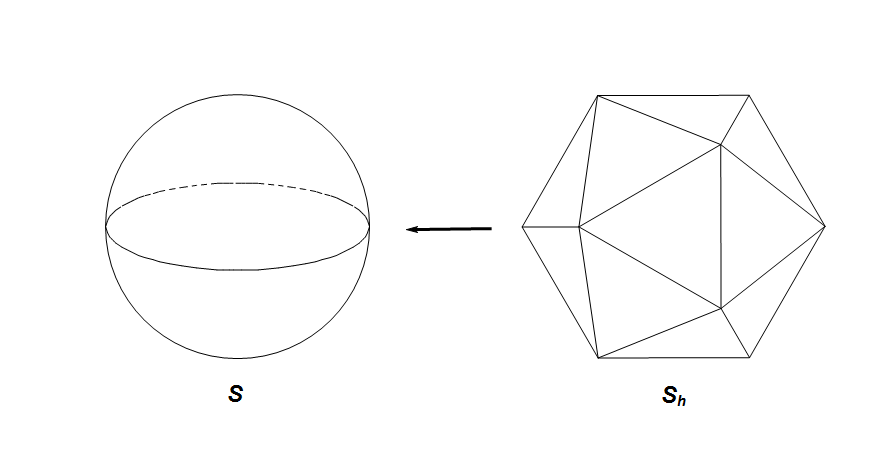
\includegraphics[scale=0.5]{./figures/picture_1.png}
\caption{}
\end{figure}
记$S_h\subset U$是由三角形单元$\tau_h$组成的多面体面,即$S_h$逼近曲面$S$,我们假设$S_h$的这些三角形单元是正则的,单元尺寸是拟一致的,且它们的顶点都在曲面$S$上.其中$\mathcal{N}_h=\left\{x_i\right\}$为$S_h$所有顶点的集合,$\mathcal{T}_h=\left\{\tau_h\right\}$ 为所有三角形单元的集合,$\mathcal{E}_h=\left\{E\right\}$为所有边的集合.对于任意的$\tau_h\in\mathcal{T}_h$,记$\boldsymbol{n}_h$为$S_h$在$\tau_h$上的单位外法向向量.对于$v_h\in C(S_h)$和$v_h|_{\tau_h}$,我们有
\begin{equation*}
\nabla_{S_h}v_h|_{\tau_h}:=\nabla v_h-(\nabla v_h\cdot\boldsymbol{n}_h)\boldsymbol{n}_h=(\boldsymbol{I}-\boldsymbol{n}_h\boldsymbol{n}^t_h)\nabla v_h=\boldsymbol{P}_h\nabla v_h\in\mathbb{R}^3
\end{equation*}
其中$\boldsymbol{P}_h=\boldsymbol{I}-\boldsymbol{n}_h\boldsymbol{n}^t_h\in\mathbb{R}^{3\times 3}$.显然$\nabla_{S_h}v_h\in(L^2(S_h))^3$

如果限制投影$\mathcal{P}_0:U\rightarrow S$到$S_h$上,就得到一个从$S_h$到$S$的连续可微的双射,仍记为$\mathcal{P}_0$.对于任意的$\tau_h\in\mathcal{T}_h$,我们可以得到一个曲面三角形$\tau:=\mathcal{P}_0(\tau_h)$,并记所有的曲面三角形集合为$\mathcal{T}_S$.

下面我们建立定义在$S$和$S_h$函数之间的关系.借助双射投影$\mathcal{P}_0$,可以由函数$v:S\rightarrow\mathbb{R}$唯一地引入另一个函数$\bar{v}:S_h\rightarrow\mathbb{R}$.对于所有的$x\in S_h$,有$\bar{v}(x)=v(\mathcal{P}_0(x))$.对于任意的$\tau_h\in\mathcal{T}_h$和函数$v\in C^1(\mathcal{P}_0(\tau_h))$,我们有
\begin{equation*}
\nabla_{S_h}\bar{v}(x)=(\boldsymbol{P}_h(\boldsymbol{I}-d\boldsymbol{H})\boldsymbol{P})(x)\nabla_{S}v(\mathcal{P}_0(x))\quad\forall x\in \tau_h.
\end{equation*}
反过来,一个函数$v_h:S_h\rightarrow\mathbb{R}$也可以唯一的引入一个函数$\tilde{v}_h:S\rightarrow\mathbb{R}$,对于所有的$x\in S$,有$\tilde{v}_h(x)=v_h(\mathcal{P}^{-1}_0(x))$.对于任意的$\tau_h\in\mathcal{T}_h$和函数$v_h\in C^1(\tau_h)$让$\tau=\mathcal{P}_0(\tau_h)$,可得
\begin{equation*}
\nabla_{S}\tilde{v}_h(x)=(\boldsymbol{I}-d\boldsymbol{H})^{-1}\left(\boldsymbol{I}-\frac{\boldsymbol{n}_h\boldsymbol{n}^t}{\boldsymbol{n}^t\boldsymbol{n}_h}\right)\nabla_{S_h}v_h(\mathcal{P}^{-1}_0(x))\quad\forall x\in\tau.
\end{equation*}

\section{曲面线性有限元}

对于三角形$\tau_h\in\mathcal{T}_h$, 记$\{\lambda_i\}$为$\tau_h$的重心坐标.   
记$\mathcal V_h$为$S_h$上的连续分片线性有限元空间, 也即对于任意的$v_h\in \mathcal V_h$和$\tau_h \in \mathcal T_h$,
$v_h$在$S_h$上连续, 且有$v_h|_{\tau_h}\in {\rm span}\{\lambda_1,\lambda_2,\lambda_3\}$.  
我们可定义$S$上的提升空间
\begin{eqnarray*}
 \tilde{V}_{h} & = &
\{\tilde{v}_{h} \, | \, \tilde{v}_{h}:=v_{h}\circ\mathcal{P}_{0}^{-1},\,
\text{其中 }v_{h}\in \mathcal V_h\},
\end{eqnarray*}
其中$\mathcal P_0: S_h \to S$为定义在(1)中的双射.   
对于$f\in L^{2}(S)$, 记
\begin{equation}\label{eq:fh}
f_{h}(x)=\bar{f}(x)-\frac{1}{|S_{h}|}\int_{S_{h}} \bar f \, \mathrm{d}\sigma_{h},
\end{equation}
其中$|S_{h}|$ 为 $ S_{h}$的总面积. 那么有
$\int_{S_{h}}f_{h}(x)\,\mathrm{d}\sigma_{h}=0$, 且下列方程存在唯一的有限元解
$u_{h}\in \mathcal V_h$, 满足$\int_{S_{h}}u_{h}\,\mathrm{d}\sigma_{h}=0$
\begin{equation*}
\int_{S_h}\nabla_{S_h}u_h\cdot\nabla_{S_h}v_h\mathrm{d}\sigma_h=\int_{S_h}f_hv_h\mathrm{d}\sigma_h\quad\forall v_h\in\mathcal{V}_h
\end{equation*}

\section{曲面高次元}
\subsection{符号说明}
\begin{table}[H]
\begin{center}
\begin{tabular}{|c|c|}
 \hline
 $S$  &$\mathbb R^3$ 空间中的曲面\\
 \hline
 $K\subset \mathbb R^2$  &二维空间中的标准单元\\
 \hline
 $\mathbf u = (u, v)^T$  &二维空间中的坐标系\\
 \hline
 $\tau_h \subset R^3$  &三维空间中的尺寸为 $h$ 的平面三角形\\  
 \hline
 $\mathbf x = (x, y, z)^T\in \tau_h$  &$\tau_h$ 上的一个点\\
 \hline
 $\mathcal P_0$  &$S$ 邻近区域到 $S$ 的投影\\
 \hline
 $\mathbf x_i,  i=1,\cdots, n_{dof}$  &$\tau_h$ 上 $p$ 次 Lagrangian 基函数对应的自由度坐标点\\
 \hline
 $\tau_p\subset \mathbb R^3$ &定义在 $\tau_h$ 上的 $p$ 次多项式曲面三角形\\
 \hline
 $ \mathbf x_p =(x_p, y_p, z_p)^T \in \tau_p$ & $\tau_p$ 上一个点的三维坐标\\
 \hline
 $\tau_S\subset \mathbb R^3$ & 把 $\tau_h$ 投影到曲面 $S$ 上的曲面三角形\\
 \hline
 $ \mathbf x_S =(x_S, y_S, z_S)^T \in \tau_S$ & $\tau_S$ 上一个点的三维坐标 \\
 \hline
 $\varphi_i(\mathbf x)$ & 定义在 $\tau_h$ 上第 $i$ 个 Lagrangian 基函数\\
 \hline 
\end{tabular}
\end{center}
\end{table}

\subsection{$\tau_h$$\quad$$\tau_p$和$\tau_s$之间关系}

对于 $\tau_p$ 上的任意一点 $\mathbf x_p$, 存在一点 $\mathbf x \in \tau_h$, 使得
\begin{equation*}
\mathbf x_p = \sum_{i=1}^{n_{dof}} \mathbf x_i \varphi_i(\mathbf x)
\end{equation*}
进一步, 存在标准参考单元 $K$ 中存在一点 $\mathbf u = (u,v)$, 可得
\begin{equation*}
\mathbf x(u,v) = \lambda_0 \mathbf x_0 + \lambda_1 \mathbf x_1 + \lambda_2 \mathbf x_2
\end{equation*}
其中 $\mathbf x_0$, $\mathbf x_1$ 和 $\mathbf x_2$ 为$\tau_h$ 的三个顶点, 
\begin{equation*}
\lambda_0 = 1- u - v,\quad\lambda_1 = u,\quad\lambda_2 = v
\end{equation*}
对于 $\tau_S$ 上的任意一点 $\mathbf x_S$, 存在 $\tau_p$ 上的一点 $\mathbf x_p$, 使得
\begin{equation*}
\mathbf x_S = \mathcal P_0(\mathbf x_p)
\end{equation*}
$\mathbf x$ 关于  $(u, v)$ 的 Jacobi 矩阵为
\begin{equation*}
\frac{\partial \mathbf x}{\partial \mathbf u} = [\mathbf x_1 - \mathbf x_0, \mathbf x_2 - \mathbf x_0]
\end{equation*}
$\mathbf x_p$ 关于 $\mathbf x$ 的 Jacobi 矩阵为
\begin{equation*}
\frac{\partial \mathbf x_p}{\partial \mathbf x} = \sum_{i=1}^{n_{dof}}
\begin{bmatrix}
x_i\nabla_{\mathbf x}\varphi_i(\mathbf x)^T\\
y_i\nabla_{\mathbf x}\varphi_i(\mathbf x)^T\\
z_i\nabla_{\mathbf x}\varphi_i(\mathbf x)^T\\
\end{bmatrix}
\end{equation*}
则 $\mathbf x_p$ 关于 $\mathbf u$ 的 Jacobi 矩阵为
\begin{equation*}
\frac{\partial \mathbf x_p}{\partial \mathbf u}=[\frac{\partial \mathbf x_p}{\partial u}, \frac{\partial \mathbf x_p}{\partial v}]=\sum_{i=1}^{n_{dof}}
\begin{bmatrix}
x_i\nabla_{\mathbf x}\varphi_i(\mathbf x)^T\\
y_i\nabla_{\mathbf x}\varphi_i(\mathbf x)^T\\
z_i\nabla_{\mathbf x}\varphi_i(\mathbf x)^T\\
\end{bmatrix}
[\mathbf x_1 - \mathbf x_0, \mathbf x_2 - \mathbf x_0]\qquad(2)
\end{equation*}
记
\begin{equation*} 
\mathrm d \mathbf x_p = \frac{\partial \mathbf x_p}{\partial \mathbf u}\mathrm d \mathbf u = \frac{\partial \mathbf x_p}{\partial u}\mathrm d u + \frac{\partial \mathbf x_p}{\partial v}\mathrm d v,
\end{equation*}
其中 $\mathrm d \mathbf u = [\mathrm d u, \mathrm d v]^T$.
进一步可得曲面三角形 $\tau_p$ 上的第一基本形式
\begin{equation*}
I = <\mathrm d \mathbf x_p, \mathrm d \mathbf x_p> = \mathrm d \mathbf u^T 
\begin{bmatrix}
g_{11} & g_{12}\\
g_{12} & g_{22}
\end{bmatrix}
\mathrm d \mathbf u
\end{equation*}
其中 
\begin{equation*}
g_{11} =<\frac{\partial \mathbf x_p}{\partial u}, \frac{\partial \mathbf x_p}{\partial u}>, 
g_{12} =<\frac{\partial \mathbf x_p}{\partial u}, \frac{\partial \mathbf x_p}{\partial v}>, 
g_{22} =<\frac{\partial \mathbf x_p}{\partial v}, \frac{\partial \mathbf x_p}{\partial v}>, 
\end{equation*}
定义$\tau_p$ 上的基函数如下
\begin{equation*}
\varphi_{p,i}(\mathbf x_p) =\varphi_i(\mathbf x) 
\end{equation*}
其中
\begin{equation*}
\mathbf x_p = \sum_{i=1}^{n_{dof}} \mathbf x_i \varphi_i(\mathbf x)
\end{equation*}
则 $\varphi_{p,i}(\mathbf x_p)$ 在 $\tau_p$ 上的切向导数定义如下:
\begin{equation*}
\nabla_{S_p} \varphi_{p,i} = \frac{\partial \mathbf x_p}{\partial \mathbf u}\begin{bmatrix}
g_{11} & g_{12}\\
g_{12} & g_{22}
\end{bmatrix}^{-1}(\frac{\partial \mathbf x}{\partial \mathbf u})^T\nabla_{S_h}\varphi_i(\mathbf x)
\end{equation*}

\subsection{$S$上曲面三角形的面积计算公式}

\begin{equation*}
\mathcal P_0(\mathbf x):=\mathbf x - d(\mathbf x)\mathbf n(\mathbf x)
\end{equation*}
对于$\mathbf x_p \in \tau_p$, 存在 $\mathbf x_S \in S$, 有
\begin{equation*}
\mathbf x_S = \mathcal P_0(\mathbf x_p)=\mathbf x_p - d(\mathbf x_p)\mathbf n(\mathbf x_p)
\end{equation*}
\begin{equation*}
\frac{\partial \mathbf x_S}{\partial\mathbf x_p} = I - d(\mathbf x_p) H(\mathbf x_p) - \mathbf n(\mathbf x_p)\mathbf n(\mathbf x_p)^T
\end{equation*}
\begin{equation*}
\frac{\partial \mathbf x_S}{\partial\mathbf u} = \frac{\partial \mathbf x_S}{\partial\mathbf x_p}\frac{\partial \mathbf x_p}{\partial\mathbf u}
\end{equation*}

\subsection{$S$上的导数计算}

考虑 $\tau_S$ 和 $\tau_p$ 的关系

则 $\mathbf x_S$ 关于 $\mathbf u$ 的 Jacobi 矩阵为
\begin{equation*}
\frac{\partial \mathbf x_S}{\partial\mathbf u} = \frac{\partial \mathbf x_S}{\partial\mathbf x_p}\frac{\partial \mathbf x_p}{\partial\mathbf u}
\end{equation*}
\begin{equation*}
\frac{\partial \mathbf x_S}{\partial\mathbf x_p} = I - d(\mathbf x_p) H(\mathbf x_p) - \mathbf n(\mathbf x_p)\mathbf n(\mathbf x_p)^T
\end{equation*}
由于
\begin{equation*}
\frac{\partial \mathbf x_p}{\partial \mathbf u}=[\frac{\partial \mathbf x_p}{\partial u}, \frac{\partial \mathbf x_p}{\partial v}]=\sum_{i=1}^{n_{dof}}
\begin{bmatrix}
x_i\nabla_{\mathbf x}\varphi_i(\mathbf x)^T\\
y_i\nabla_{\mathbf x}\varphi_i(\mathbf x)^T\\
z_i\nabla_{\mathbf x}\varphi_i(\mathbf x)^T\\
\end{bmatrix}
[\mathbf x_1 - \mathbf x_0, \mathbf x_2 - \mathbf x_0]
\end{equation*}
即,很容易计算
\begin{equation*}
\frac{\partial \mathbf x_S}{\partial\mathbf u}
\end{equation*}
进一步可得到曲面 $\tau_S$ 上的第一基本形式
记
\begin{equation*} 
\mathrm d \mathbf x_S = \frac{\partial \mathbf x_S}{\partial \mathbf u}\mathrm d \mathbf u = \frac{\partial \mathbf x_S}{\partial u}\mathrm d u + \frac{\partial \mathbf x_S}{\partial v}\mathrm d v,
\end{equation*}
其中
\begin{equation*}
\begin{aligned}
\mathrm d \mathbf x_S & = \frac{\partial \mathbf x_S}{\partial \mathbf u}\mathrm d \mathbf u \\
& =\frac{\partial \mathbf x_S}{\partial\mathbf x_p}\frac{\partial \mathbf x_p}{\partial\mathbf u}\mathrm d \mathbf u \\
& = \frac{\partial \mathbf x_S}{\partial\mathbf x_p}\frac{\partial \mathbf x_p}{\partial u}\mathrm d u + \frac{\partial \mathbf x_S}{\partial\mathbf x_p}\frac{\partial \mathbf x_p}{\partial v}\mathrm d v\\
\end{aligned}
\end{equation*}
故
\begin{equation*}
\begin{aligned}
\frac{\partial \mathbf x_S}{\partial u} &= \frac{\partial \mathbf x_S}{\partial\mathbf x_p}\frac{\partial \mathbf x_p}{\partial u}\\
\frac{\partial \mathbf x_S}{\partial v} &= \frac{\partial \mathbf x_S}{\partial\mathbf x_p}\frac{\partial \mathbf x_p}{\partial v}
\end{aligned}
\end{equation*}
\begin{equation*}
I = <\mathrm d \mathbf x_S, \mathrm d \mathbf x_S> = \mathrm d \mathbf u^T 
\begin{bmatrix}
g'_{11} & g'_{12}\\
g'_{12} & g'_{22}
\end{bmatrix}
\mathrm d \mathbf u
\end{equation*}
其中 
\begin{equation*}
g'_{11} =<\frac{\partial \mathbf x_S}{\partial u}, \frac{\partial \mathbf x_S}{\partial u}>, 
g'_{12} =<\frac{\partial \mathbf x_S}{\partial u}, \frac{\partial \mathbf x_S}{\partial v}>, 
g'_{22} =<\frac{\partial \mathbf x_S}{\partial v}, \frac{\partial \mathbf x_S}{\partial v}>, 
\end{equation*}
定义$\tau_S$ 上的基函数如下
\begin{equation*}
\varphi_{S,i}(\mathbf x_S) =\varphi_{i}(\mathbf x) 
\end{equation*}
其中
\begin{equation*}
\mathbf x_S = \sum_{i=1}^{n_{dof}} \mathbf x_i \varphi_{i}(\mathbf x) 
\end{equation*}
则 $\varphi_{S,i}(\mathbf x_S)$ 在 $\tau_S$ 上的导数定义如下:
\begin{equation*}
\nabla_{S_S} \varphi_{S,i} = \frac{\partial \mathbf x_S}{\partial \mathbf u}\begin{bmatrix}
g'_{11} & g'_{12}\\
g'_{12} & g'_{22}
\end{bmatrix}^{-1}(\frac{\partial \mathbf x}{\partial \mathbf u})^T\nabla_{S_h}\varphi_{i}(\mathbf x) 
\end{equation*}
设 $w(\mathbf x_S)$ 是定义在 $S$ 上的函数, 利用投影可以定义 $S_p$ 上函数 
\begin{equation*}
\hat w(\mathbf x_p) = w(\mathcal P_0(x_p))
\end{equation*}
下面讨论如何计算 $\nabla_{S_p} w$. 
\begin{equation*}
\nabla_{S_p} \hat w(\mathbf x_p) = \frac{\partial \mathbf x_p}{\partial \mathbf u}\begin{bmatrix}
g_{11} & g_{12}\\
g_{12} & g_{22}
\end{bmatrix}^{-1}
\begin{pmatrix}
\hat w_u \\ \hat w_v
\end{pmatrix}
\end{equation*}
\begin{equation*}
\begin{pmatrix}
\hat w_u \\ \hat w_v
\end{pmatrix}
= (\frac{\partial \mathbf x_S}{\partial \mathbf u})^T \nabla_{\mathbf x_S} w(x_S)
\end{equation*}












\nocite{*}
\bibliography{}
\end{document}


